%%%%%%%%%%%%%%%%%%%%%%%%%%%%%%%%%%%%%%%%%%%%%%%%%%%%%%%%%%%%%%%%%%%%%%
% How to use writeLaTeX: 
%
% You edit the source code here on the left, and the preview on the
% right shows you the result within a few seconds.
%
% Bookmark this page and share the URL with your co-authors. They can
% edit at the same time!
%
% You can upload figures, bibliographies, custom classes and
% styles using the files menu.
%
% If you're new to LaTeX, the wikibook is a great place to start:
% http://en.wikibooks.org/wiki/LaTeX
%
%%%%%%%%%%%%%%%%%%%%%%%%%%%%%%%%%%%%%%%%%%%%%%%%%%%%%%%%%%%%%%%%%%%%%%
\documentclass{tufte-book}

\hypersetup{colorlinks}% uncomment this line if you prefer colored hyperlinks (e.g., for onscreen viewing)

%%
% Book metadata
\title{Notes on Physical Geodesy}
\publisher{Publisher of This Book}

%%
% If they're installed, use Bergamo and Chantilly from www.fontsite.com.
% They're clones of Bembo and Gill Sans, respectively.
%\IfFileExists{bergamo.sty}{\usepackage[osf]{bergamo}}{}% Bembo
%\IfFileExists{chantill.sty}{\usepackage{chantill}}{}% Gill Sans

%\usepackage{microtype}

%%
% Just some sample text
\usepackage{lipsum}
\usepackage{amsmath}
\usepackage{amssymb}
%%
% For nicely typeset tabular material
\usepackage{booktabs}

%%
% For graphics / images
\usepackage{graphicx}
\setkeys{Gin}{width=\linewidth,totalheight=\textheight,keepaspectratio}
\graphicspath{{graphics/}}

% The fancyvrb package lets us customize the formatting of verbatim
% environments.  We use a slightly smaller font.
\usepackage{fancyvrb}
\fvset{fontsize=\normalsize}

%%
% Prints argument within hanging parentheses (i.e., parentheses that take
% up no horizontal space).  Useful in tabular environments.
\newcommand{\hangp}[1]{\makebox[0pt][r]{(}#1\makebox[0pt][l]{)}}

%%
% Prints an asterisk that takes up no horizontal space.
% Useful in tabular environments.
\newcommand{\hangstar}{\makebox[0pt][l]{*}}

%%
% Prints a trailing space in a smart way.
\usepackage{xspace}

%%
% Some shortcuts for Tufte's book titles.  The lowercase commands will
% produce the initials of the book title in italics.  The all-caps commands
% will print out the full title of the book in italics.
\newcommand{\vdqi}{\textit{VDQI}\xspace}
\newcommand{\ei}{\textit{EI}\xspace}
\newcommand{\ve}{\textit{VE}\xspace}
\newcommand{\be}{\textit{BE}\xspace}
\newcommand{\VDQI}{\textit{The Visual Display of Quantitative Information}\xspace}
\newcommand{\EI}{\textit{Envisioning Information}\xspace}
\newcommand{\VE}{\textit{Visual Explanations}\xspace}
\newcommand{\BE}{\textit{Beautiful Evidence}\xspace}

\newcommand{\TL}{Tufte-\LaTeX\xspace}

% Prints the month name (e.g., January) and the year (e.g., 2008)
\newcommand{\monthyear}{%
  \ifcase\month\or January\or February\or March\or April\or May\or June\or
  July\or August\or September\or October\or November\or
  December\fi\space\number\year
}


% Prints an epigraph and speaker in sans serif, all-caps type.
\newcommand{\openepigraph}[2]{%
  %\sffamily\fontsize{14}{16}\selectfont
  \begin{fullwidth}
  \sffamily\large
  \begin{doublespace}
  \noindent\allcaps{#1}\\% epigraph
  \noindent\allcaps{#2}% author
  \end{doublespace}
  \end{fullwidth}
}

% Inserts a blank page
\newcommand{\blankpage}{\newpage\hbox{}\thispagestyle{empty}\newpage}

\usepackage{units}

\usepackage{graphicx}
% Typesets the font size, leading, and measure in the form of 10/12x26 pc.
\newcommand{\measure}[3]{#1/#2$\times$\unit[#3]{pc}}

% Macros for typesetting the documentation
\newcommand{\hlred}[1]{\textcolor{Maroon}{#1}}% prints in red
\newcommand{\hangleft}[1]{\makebox[0pt][r]{#1}}
\newcommand{\hairsp}{\hspace{1pt}}% hair space
\newcommand{\hquad}{\hskip0.5em\relax}% half quad space
\newcommand{\TODO}{\textcolor{red}{\bf TODO!}\xspace}
\newcommand{\ie}{\textit{i.\hairsp{}e.}\xspace}
\newcommand{\eg}{\textit{e.\hairsp{}g.}\xspace}
\newcommand{\na}{\quad--}% used in tables for N/A cells
\providecommand{\XeLaTeX}{X\lower.5ex\hbox{\kern-0.15em\reflectbox{E}}\kern-0.1em\LaTeX}
\newcommand{\tXeLaTeX}{\XeLaTeX\index{XeLaTeX@\protect\XeLaTeX}}
% \index{\texttt{\textbackslash xyz}@\hangleft{\texttt{\textbackslash}}\texttt{xyz}}
\newcommand{\tuftebs}{\symbol{'134}}% a backslash in tt type in OT1/T1
\newcommand{\doccmdnoindex}[2][]{\texttt{\tuftebs#2}}% command name -- adds backslash automatically (and doesn't add cmd to the index)
\newcommand{\doccmddef}[2][]{%
  \hlred{\texttt{\tuftebs#2}}\label{cmd:#2}%
  \ifthenelse{\isempty{#1}}%
    {% add the command to the index
      \index{#2 command@\protect\hangleft{\texttt{\tuftebs}}\texttt{#2}}% command name
    }%
    {% add the command and package to the index
      \index{#2 command@\protect\hangleft{\texttt{\tuftebs}}\texttt{#2} (\texttt{#1} package)}% command name
      \index{#1 package@\texttt{#1} package}\index{packages!#1@\texttt{#1}}% package name
    }%
}% command name -- adds backslash automatically
\newcommand{\doccmd}[2][]{%
  \texttt{\tuftebs#2}%
  \ifthenelse{\isempty{#1}}%
    {% add the command to the index
      \index{#2 command@\protect\hangleft{\texttt{\tuftebs}}\texttt{#2}}% command name
    }%
    {% add the command and package to the index
      \index{#2 command@\protect\hangleft{\texttt{\tuftebs}}\texttt{#2} (\texttt{#1} package)}% command name
      \index{#1 package@\texttt{#1} package}\index{packages!#1@\texttt{#1}}% package name
    }%
}% command name -- adds backslash automatically
\newcommand{\docopt}[1]{\ensuremath{\langle}\textrm{\textit{#1}}\ensuremath{\rangle}}% optional command argument
\newcommand{\docarg}[1]{\textrm{\textit{#1}}}% (required) command argument
\newenvironment{docspec}{\begin{quotation}\ttfamily\parskip0pt\parindent0pt\ignorespaces}{\end{quotation}}% command specification environment
\newcommand{\docenv}[1]{\texttt{#1}\index{#1 environment@\texttt{#1} environment}\index{environments!#1@\texttt{#1}}}% environment name
\newcommand{\docenvdef}[1]{\hlred{\texttt{#1}}\label{env:#1}\index{#1 environment@\texttt{#1} environment}\index{environments!#1@\texttt{#1}}}% environment name
\newcommand{\docpkg}[1]{\texttt{#1}\index{#1 package@\texttt{#1} package}\index{packages!#1@\texttt{#1}}}% package name
\newcommand{\doccls}[1]{\texttt{#1}}% document class name
\newcommand{\docclsopt}[1]{\texttt{#1}\index{#1 class option@\texttt{#1} class option}\index{class options!#1@\texttt{#1}}}% document class option name
\newcommand{\docclsoptdef}[1]{\hlred{\texttt{#1}}\label{clsopt:#1}\index{#1 class option@\texttt{#1} class option}\index{class options!#1@\texttt{#1}}}% document class option name defined
\newcommand{\docmsg}[2]{\bigskip\begin{fullwidth}\noindent\ttfamily#1\end{fullwidth}\medskip\par\noindent#2}
\newcommand{\docfilehook}[2]{\texttt{#1}\index{file hooks!#2}\index{#1@\texttt{#1}}}
\newcommand{\doccounter}[1]{\texttt{#1}\index{#1 counter@\texttt{#1} counter}}

% Generates the index
\usepackage{makeidx}
\makeindex

\begin{document}

% Front matter
\frontmatter

% r.1 blank page
\blankpage

% v.2 epigraphs



% r.3 full title page
\maketitle


% v.4 copyright page
\newpage
\begin{fullwidth}
~\vfill
\thispagestyle{empty}
\setlength{\parindent}{0pt}
\setlength{\parskip}{\baselineskip}
Copyright \copyright\ \the\year\ \thanklessauthor

\par\smallcaps{Published by \thanklesspublisher}

\par\smallcaps{tufte-latex.googlecode.com}

\par Licensed under the Apache License, Version 2.0 (the ``License''); you may not
use this file except in compliance with the License. You may obtain a copy
of the License at \url{http://www.apache.org/licenses/LICENSE-2.0}. Unless
required by applicable law or agreed to in writing, software distributed
under the License is distributed on an \smallcaps{``AS IS'' BASIS, WITHOUT
WARRANTIES OR CONDITIONS OF ANY KIND}, either express or implied. See the
License for the specific language governing permissions and limitations
under the License.\index{license}

\par\textit{First printing, \monthyear}
\end{fullwidth}

% r.5 contents
\tableofcontents

\listoffigures

\listoftables

% r.7 dedication
\cleardoublepage
~\vfill
\begin{doublespace}
\noindent\fontsize{18}{22}\selectfont\itshape
\nohyphenation
Dedicated to those who appreciate \LaTeX{} 
and the work of \mbox{Edward R.~Tufte} 
and \mbox{Donald E.~Knuth}.
\end{doublespace}
\vfill
\vfill


% r.9 introduction
\cleardoublepage
\chapter*{Introduction}
This work is very beta. A lot of errors are expected.
%%
% Start the main matter (normal chapters)
\mainmatter


\chapter{Laplace's Equation}
We will begin our discussion about Laplace's equation. 

\begin{equation}
	\label{eqn:laplace}
	\triangle V = 0
\end{equation}
and notice that this differential operator $\triangle(\cdot)$ is just \(\nabla\cdot\nabla(\cdot)\). Solving Laplace's equation is not easy. The common way of doing that is solving it at some coordinate system; Cartesian system, spherical system, etc. In physical geodesy, we use Laplace's equation to compute the potential of a field i.e., potential of the gravity field. From that potential, one can compute other functions e.g., gravity disturbance, geoid height, gravity anomaly, etc. That's why we are studying it.

\section{Laplace's equation in Cartesian Coordinate System}

Recall that from Eqn. \eqref{eqn:laplace}, Laplace's equation is
\begin{equation*}
\triangle V = 0
\end{equation*}, replacing $V$ by its values yields,
\begin{equation*}
\nabla \cdot \nabla V = \left(\frac{\partial^2}{\partial X^2}\cdot\frac{\partial^2}{\partial Y^2}\cdot\frac{\partial^2}{\partial Z^2}\right)
\end{equation*}. So, we basically using the dot product property to separate these functions. Applying the chain rule to compute the second derivative of these functions give us,
\begin{equation}
\label{eqn:chain-rule-laplace}
\triangle V = \frac{\partial^2 X}{\partial x^2} YZ + \frac{\partial^2 Y}{\partial x^2} XY + \frac{\partial^2 Z}{\partial x^2} YX = 0
\end{equation}. 
And because we want to separate between the $x$ in the derivative, and that of the vector, let us rearrange the equation as following

\begin{equation}
	\label{eqn:laplace-separation}
	\frac{\partial^2 X(\cdot)}{\partial x^2} YZ + \frac{\partial^2 Y(\cdot)}{\partial x^2} XY + \frac{\partial^2 Z(\cdot)}{\partial x^2} YX = 0
\end{equation}
Because each of these variables $(X, Y, Z)$ are actually a function. Now let us divide Eqn. \eqref{eqn:laplace-separation} by \(XYZ\), to get

\begin{equation}
\label{eqn:laplace-divided}
\frac{\frac{\partial^2 X}{\partial x^2}}{X(\cdot)} + \frac{\frac{\partial^2 Y}{\partial y^2}}{Y(\cdot)} + \frac{\frac{\partial^2 Z}{\partial z^2}}{Z(\cdot)} = 0
\end{equation}
 This is indeed a partial ordinary differential equation. In order for the solution to be true for all \(X, Y, Z\), each of these terms should be a constant \footnote{Well, as you can see we are taking the derivative for these functions. For the answer to be equals to zero, each of these terms should be a constant != 0. You get the idea?}. For the base solution for this differential equation, we choose 
 Let us rearrange Eqn. \eqref{eqn:laplace-divided} to be like the following, and only taking the \(X\)
part,
\begin{equation}
	\label{eqn:deriving-laplace-x-part}
	\frac{\partial^2 X}{\partial x^2} = -k_1^2 X,\   \text{where $k_1$ is a constant}
\end{equation}
and similarly for the $Y(\cdot)$ and $Z(\cdot)$ part,
\begin{equation}
\label{eqn:deriving-laplace-y-part}
\frac{\partial^2 Y}{\partial y^2} = -k_2^2 Y,
\end{equation}
\begin{equation}
\frac{\partial^2 Z}{\partial y^2} = (k_1^2+k_2^2) Z
\end{equation}

For the base solution \footnote{Other base solutions can be chosen e.g., \(\sin mx, \cos my\). This solution is a common one in the literature. } we have,

\begin{eqnarray}
\label{eqn:base-solution}
X(x) &= e^{\pm ik_1 x},\\
Y(y) &= e^{\pm ik_2 y},\\
Z(z) &= e^{\pm z\sqrt{k_1^2 + k_2^2}}
\end{eqnarray}

to get,
\begin{equation}
V_{k_1, k_2} = e^{\left(\pm (ik_1 x + i k_2 y) \pm z \sqrt{k_1^2 + k_2^2}\right)}
\end{equation}.
And recall that from the beginning we have restricted ourselves in a "Cartesian system", well the reason for that is because we want to have some boundary values to solve our problem! Defining the boundary condition for this BVP might be a little bit hard. In Fig. \ref{fig:shorebox}, we have a box with dimensions of $L_1 ,L_2, L_3$, we have these set of conditions,

\begin{eqnarray}
V(0, Y, Z) = V(X, 0, Z) = V(X, Y, 0) &= 0\\
V(L_1, Y, Z) = V(X, L_2, Z) &= 0\\
V(X, Y, L_3) &= f(X, Y)
\end{eqnarray}

Then, the boundary conditions can be rewritten as follows,
\begin{eqnarray}
X(0) = X(L_1) &= 0\\
Y(0) = Y(L_2) &= 0\\
Z(0) &= 0
\end{eqnarray}

\begin{figure}
	\centering
	\label{fig:shorebox}
	\caption{Think of this box as our world e.g., the Earth. The size of this box is L. Credits of Professor D. K. Ghosh.}
	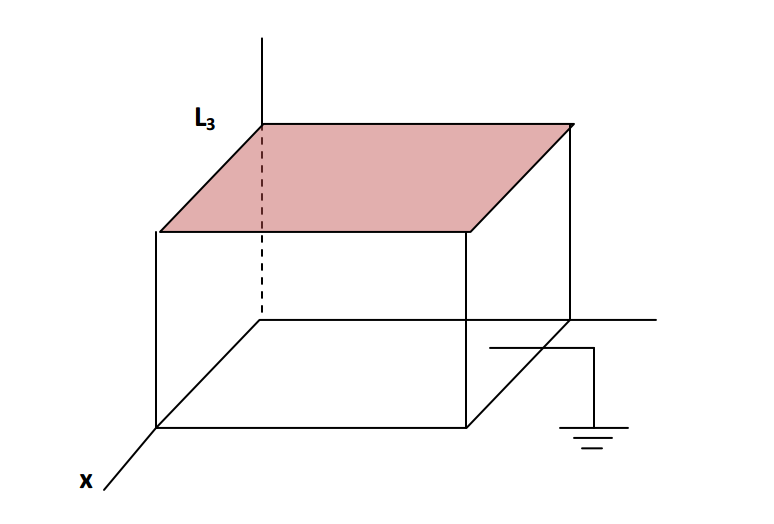
\includegraphics{./Figure/fig-shorebox.png}
\end{figure}

It follows that the only $k_1, k_2$ that fits these conditions are,
\begin{eqnarray}
k_1 &= \frac{\pi j}{L}\\
k_2 &= \frac{\pi k}{L}
\end{eqnarray}

and the sine functions are the only suitable functions for this. 

\begin{equation}
\label{eqn:general-solution}
	V_{i, k} (x, y, z) = \sin (\pi \frac{j x}{L}) \sin (\pi \frac{k y}{L})\ e^{\left( \pm \pi \sqrt{(j^2+k^2)}\frac{z}{L}\right)}
\end{equation}

This solution may now be generalized for different values of $j, k = \pm 1, \pm 2 \pm 3 \ldots$. Notice that the sine of zero is zero, in this case for $j,k = 0$ the solution is $0$. Also, for $n \in \mathbb{R}$ the solution is identical. The zero-level for Eqn. \eqref{eqn:general-solution}, is the familiar (?) Fourier sine expansion,

\begin{eqnarray}
\label{eqn:fourier-sine-expansion}
V(x, y, 0) = \sum_{j=1}^{\infty}\sum_{k=1}^{\infty} \upsilon_{jk} \sin \left( \pi \frac{jx}{L}\right) \sin\left( \pi \frac{k y}{L}\right)
\end{eqnarray}


%%
% The back matter contains appendices, bibliographies, indices, glossaries, etc.







\backmatter

\bibliography{sample-handout}
\bibliographystyle{plainnat}


\printindex

\end{document}
